\section{model fitting}

\begin{figure}
\centering
  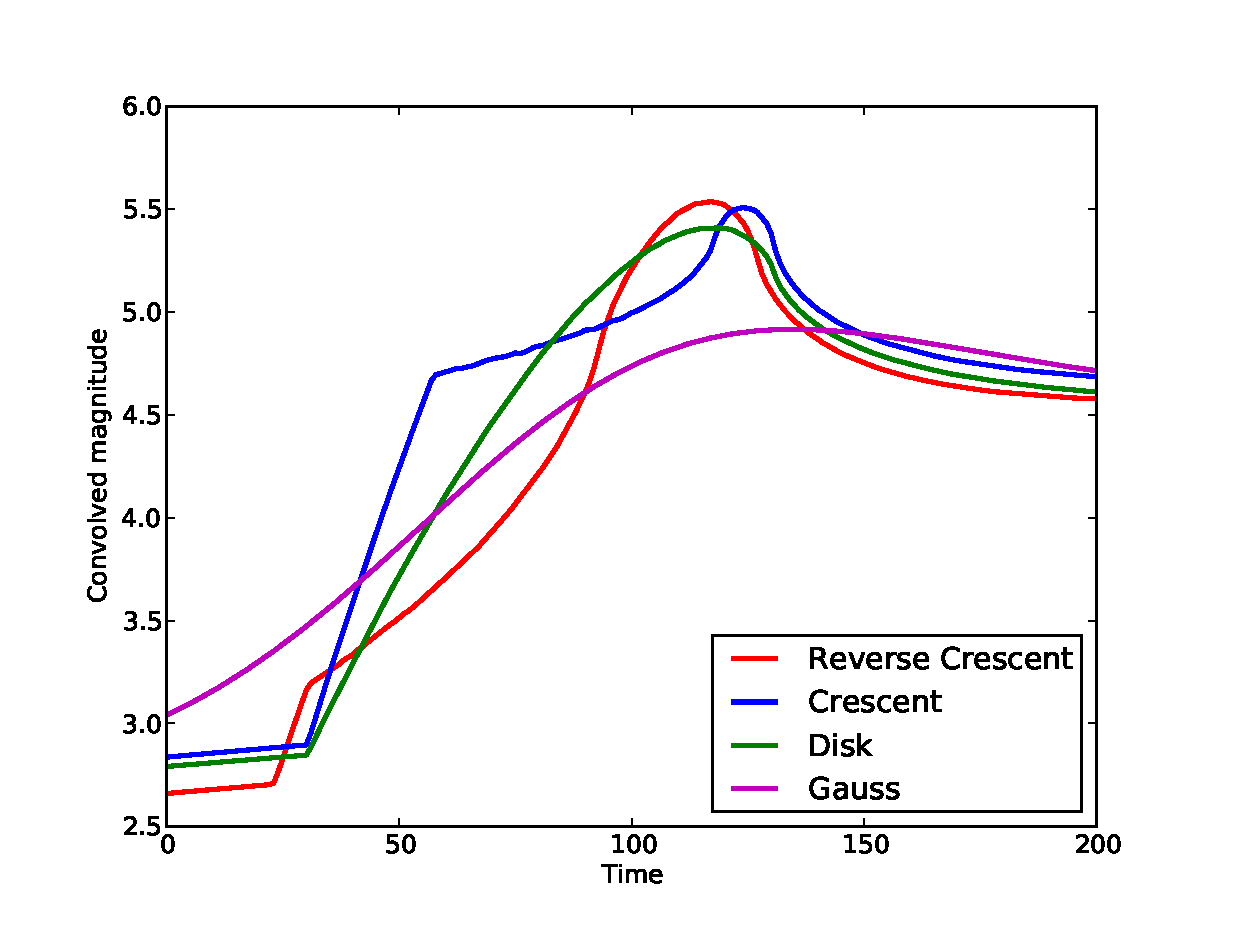
\includegraphics[width=0.95\hsize]{plots/data.eps}
\caption{\label{fig:datafitting} data}
\end{figure}


\begin{figure}
\centering
  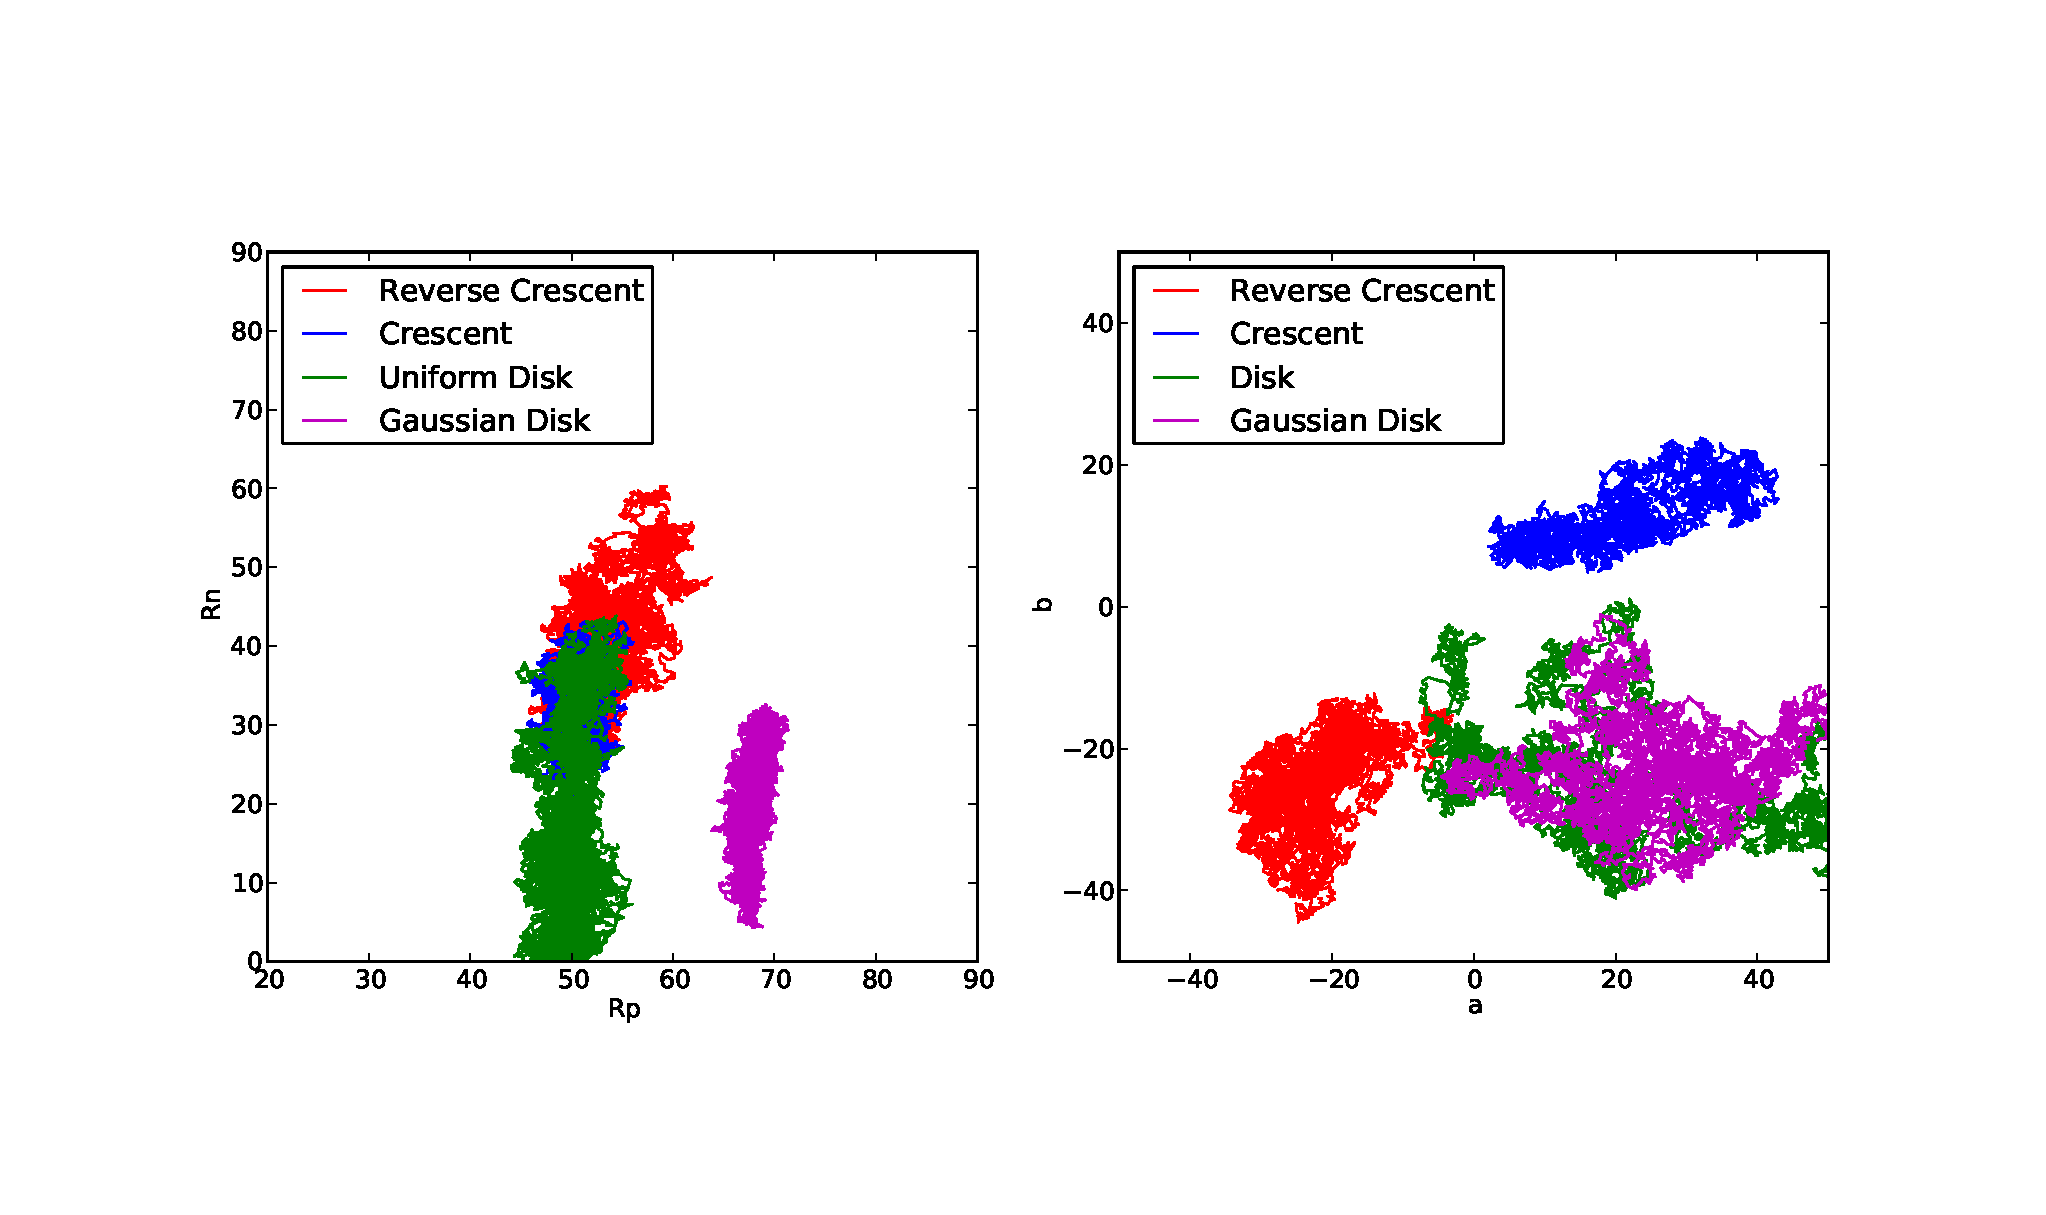
\includegraphics[width=0.95\hsize]{plots/image.eps}
  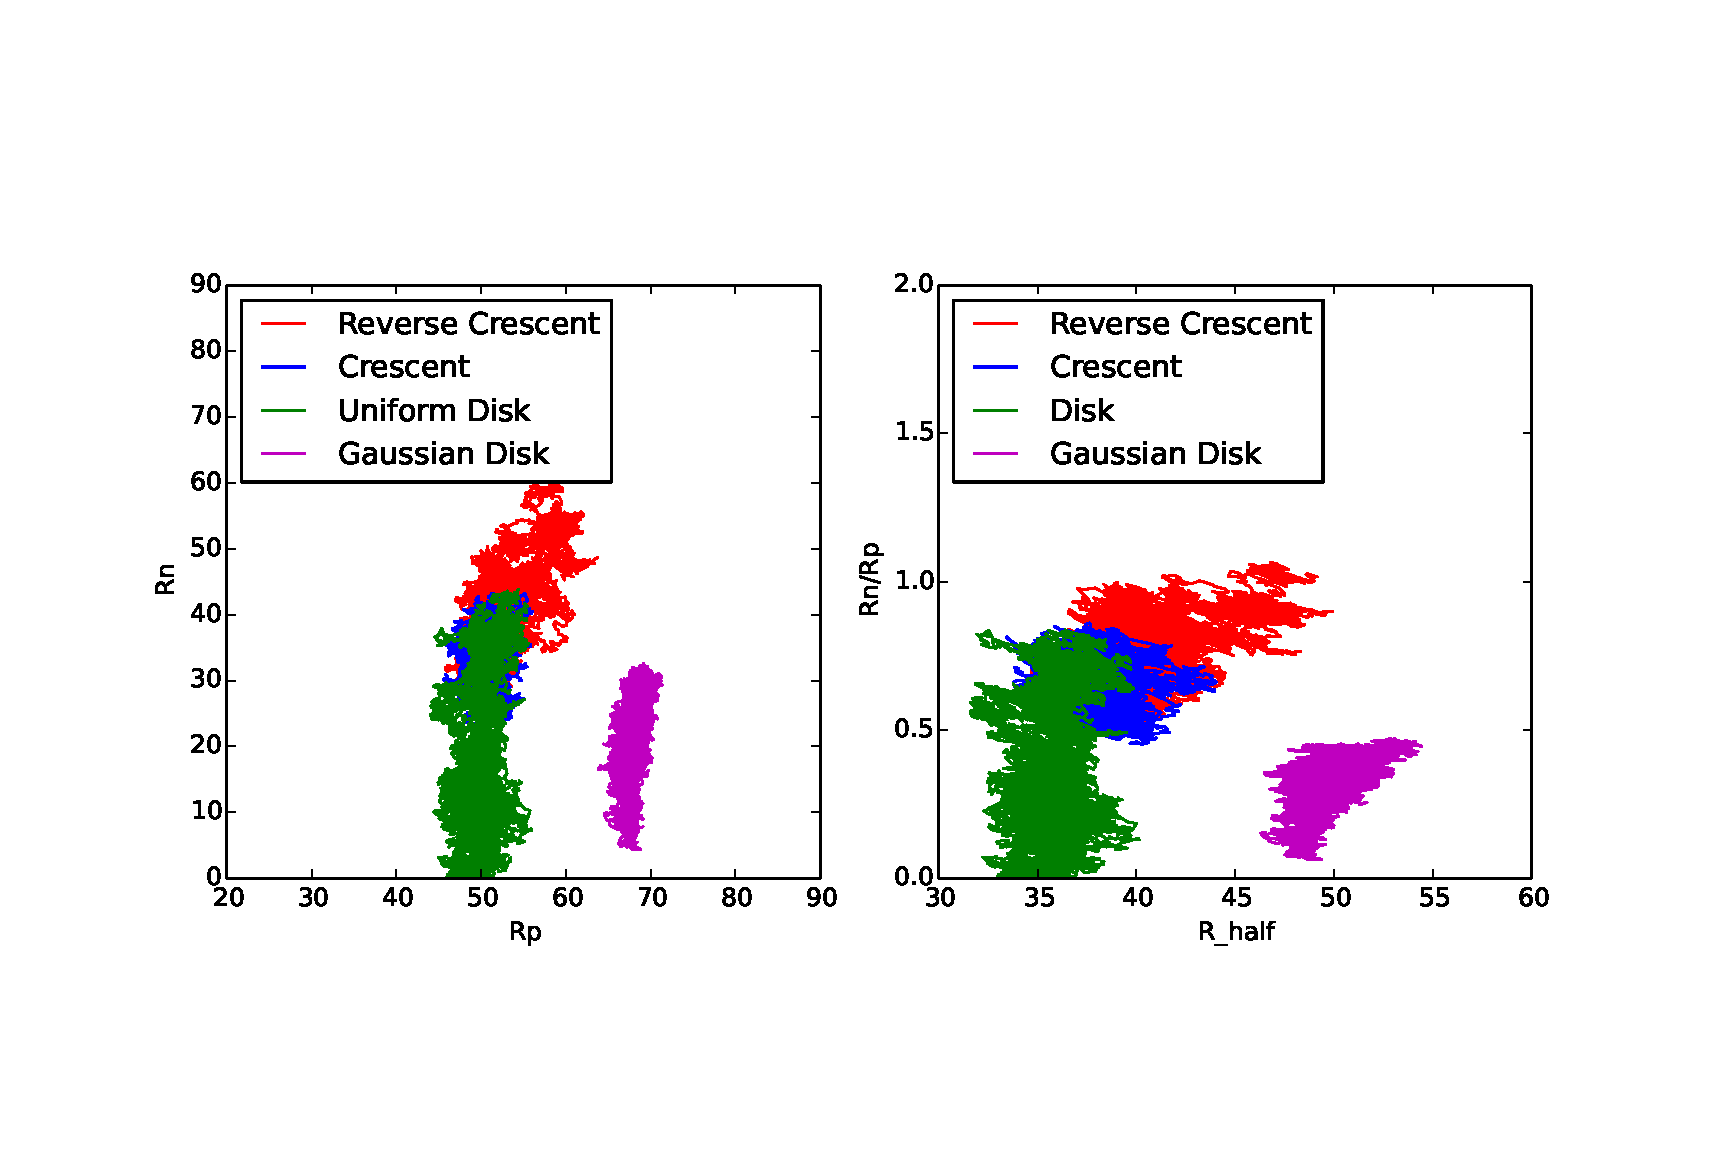
\includegraphics[width=0.95\hsize]{plots/image2.eps}
\caption{\label{fig:mcmc} Model Fitting}
\end{figure}


In this section, we attempt to recover the crescent model parameters ($R_p, R_n, a, b$) from the given dataset generated by different source models - crescent, uniform-disk and Gaussian-disk for a given set of parameters. The form of light curves in each source model can be seen in figure \ref{fig:datafitting}. There is a fourth dataset included, which is generated through the crescent source model crossing the caustic (see the magnification map) for the second time but in reverse order (indicated as reverse fold in figure \ref{fig:datafitting}). This dataset resembles an arbitary caustic crossing of a crescent shape source including noise.  The data assumed was very  ideal, including 200 different data points at regular interval of time. The aim of this exercise was to explore the degeneracies in  various crescent parameters and recover the correct fiducial model assumed. Also, it can be inferred if one can simply distinguish between circularly symmetric and asymmetric sources or uniform and Gaussian sources.


We explored the parameter space (for crescent model) using Markov-Chain Monte-Carlo (MCMC), assuming the errors on light curve data point are Gaussian distributed and about 10 percent of the light curve data point. Following the same color scheme (as in figure \ref{fig:datafitting}), figure \ref{fig:mcmc} shows the raw MCMC for each case, top row resembles the real parameter space that was explored, however, the bottom row shows the MCMC in the so-called 'derived parameters' which are more intuitive in their physical meaning.

In the first case, we tried to fit the crescent data (blue line in figure \ref{fig:datafitting}) with our crescent model parameters. The maximum likelihood (or the best fit) overlaps well with the fiducial values of the parameters assumed to generate the data. Also a degeneracy between the parameters is noticeable, particularly between $a$ and $b$. The overall shape of the crescent, the outer and inner radius, can be very well constrained.

In second case, we tried to fit the reverse crescent data (red line in figure \ref{fig:datafitting}). As already mentioned, this case resemble an arbitary caustic crossing including noise, it is the most interesting case study. We see the similar degeneracies in $a$ and $b$ as in the previous case, however, in the parameter space both the parameters changes the sign. This is also intuitive as we are assuming the motion of the source in reverse direction as compared to the previous case. On the other hand, $R_p$ and $R_n$ are ver well constrained and overlap nicely with the previous case (see red curves in figure \ref{fig:mcmc}). Even for $R_p$ and $R_n$ the maximum likelihood does not exactly co-incide with the fiducial values, but it is in the neighbourhod and  within 1-$\sigma$ errors.

In third case, we shifted our analysis towards sources with circularly symmetric brighness profile. First, we tested a uniform disk case (green in figure \ref{fig:datafitting} and \ref{fig:mcmc}). Also, one can assume the uniform disk as a special case of the crescent model with $R_n = 0$. In such scenario, one should expect the maximum likelihood for any arbitary $a$ and $b$, and $R_n = 0$. This is exactly what one can see in figure \ref{fig:mcmc}. The overall size of the source can be recovered as $R_p$ is well constrained in this case.

In our last case, we tested another circularly symmetric source but with Gaussian brightness profile (Gaussian disk, magenta color in figure \ref{fig:datafitting} and \ref{fig:mcmc}). One can easily notice in figure \ref{fig:mcmc}, that the correct crescent parameters cannot be recovered. 

In the last two cases (with circularly symmetric sources), $R_n$ can assume a long range of values or it is weakly constrained, however,  $R_p$ is very well constrained. This outer radius $R_p$ can be very well recovered in the first case (uniform disk) but assumed a larger value for Gaussian disk case. If one can imagine total brighness profile should be conserved, this observation is intuitive.

We finally conclude the following:
\begin{enumerate}
 \item If a source have a crescent shape, it can be well recovered. 
 \item If a source have circularly symmetric brighness profile, it can also be identified by looking at the parameter space.
 \item It is also possible to distinguish if the circularly symmetric source has a uniform brightness profile or a Gaussian brightness profile.

 
\end{enumerate}